%\documentclass[a4paper]{article}
%\usepackage[utf8]{inputenc}
\usepackage[spanish, es-tabla, es-noshorthands]{babel}
\usepackage[table,xcdraw,dvipsnames]{xcolor}
\usepackage[a4paper, footnotesep=1.25cm, headheight=1.25cm, top=2.54cm, left=2.54cm,
 bottom=2.54cm, right=2.54cm]{geometry}
%\geometry{showframe}
 \usepackage[normalem]{ulem}
 \useunder{\uline}{\ul}{}

%VERIFICAR EL HEAD Y EL FOOT EN
%https://ctan.dcc.uchile.cl/macros/latex/contrib/geometry/geometry.pdf

%Paquetes varios:
\usepackage{verbatimbox}

%\usepackage{wrapfig}			%Wrap figure in text
\usepackage[export]{adjustbox}	%Move images
\usepackage{changepage}			%Move tables
\usepackage{todonotes}

\usepackage{tikz}
\usepackage{amsmath}
\usepackage{amsfonts}
\usepackage{amssymb}
\usepackage{float}
\usepackage[graphicx]{realboxes}
\usepackage{caption}
\usepackage{subcaption}
\usepackage{multicol}
\usepackage{multirow}
\setlength{\doublerulesep}{\arrayrulewidth}
%\usepackage{booktabs}

\usepackage{array}
\newcolumntype{C}[1]{>{\centering\let\newline\\\arraybackslash\hspace{0pt}}m{#1}}
%\usepackage[american]{circuitikz}
\usetikzlibrary{calc}
\usepackage{fancyhdr}
\usepackage{units} 

\usepackage{colortbl}
%\usepackage{sectsty}
%\usepackage{unicode-math}

%FONTS (IMPORTANTE): Compilar en XeLaTex o LuaLaTeX
\usepackage{anyfontsize}	%Font size
\usepackage{fontspec}		%Font type
%Si sigue sin andar comentar \usepackage[utf8]{inputenc}
%https://ctan.dcc.uchile.cl/macros/unicodetex/latex/fontspec/fontspec.pdf
%https://www.overleaf.com/learn/latex/XeLaTeX

%Path para imagenes para trabajar en subarchivos
\graphicspath{{../Resumen/}{../Referencias/}{../Apendice/}{../Descripción de la Empresa/}{../Tareas del Alumno/}{../Conclusiones/}{../Herramientas Empleadas/}}

%Definiciones de nuevos comandos y colores
%COLORES:
\definecolor{AzulFoot}{rgb}{0.682,0.809,0.926}	%RGB	%{174,206,235}
\definecolor{AzulInfo}{rgb}{0.180,0.455,0.710}	%RGB	%{46,116,181}
\definecolor{AzulTable}{rgb}{0.302,0.507,0.871}	%RGB	%{68,114,196}
\definecolor{PName}{rgb}{0.353,0.353,0.353}		%RGB	%{90,90,90}
\definecolor{mygreen}{rgb}{28,172,0} % color values Red, Green, Blue
\definecolor{mylilas}{rgb}{170,55,241}

%Change Font Size

% #1 = size, #2 = text
\newcommand{\setparagraphsize}[2]{{\fontsize{#1}{6}\selectfont#2 \par}}		%Cambia el size de todo el parrafo
\newcommand{\setlinesize}[2]{{\fontsize{#1}{6}\selectfont#2}}				%Cambia el font de una oración

%IMAGE IN TABLE:			%Ejemplo: \includeintable{.3}{ImagenesFactibilidad/pend}
\renewcommand\fbox{\fcolorbox{white}{white}}
\setlength{\fboxrule}{0pt}	%padding thickness
\setlength{\fboxsep}{4pt}	%border thickness
\newcommand{\includeintable}[2]{	
	\fbox{
		\begin{minipage}{#1\textwidth}
        	\includegraphics[width=\linewidth]{#2}
    	\end{minipage}
	}
}

%LINK IN REF
\newcommand{\reflink}[1]{		%LINK
	\href{#1}{#1}
}

%NOTAS:
\newcommand{\note}[1]{		%RED BIG NOTE (TODO)
	\begin{center}
		\huge{ \textcolor{red}{#1} }
	\end{center}
}

\newcommand{\lnote}[1]{{\fontsize{14}{6}\selectfont\textcolor{green}{#1}}}	%Notas pequeñas

\newcommand{\observacion}[2]{  \ifnumequal{1}{#1}{ { \todo[inline,backgroundcolor=red!25,bordercolor=red!100]{\textbf{Observación: #2}} } }{  }  }

\newcommand{\red}[1]{\textcolor{red}{#1}}

\newcommand{\TBD}{\textcolor{red}{(TBD) }}
\newcommand{\tbd}{\textcolor{red}{(TBD) }}

\newcommand{\TBC}{\textcolor{red}{(TBC) }}
\newcommand{\tbc}{\textcolor{red}{(TBC) }}

\newcommand{\quotes}[1]{``#1''}
\newcommand{\q}[1]{``#1''}

\newcommand{\ip}{192.168.0.10:1880}
\newcommand{\ipadmin}{192.168.0.10:1880/admin}

% Comandos para agregar elementos en tablas de acronimos y definiciones
\newcommand{\addacronym}[2]{\textbf{#1} & \begin{tabular}[l]{@{}l@{}}#2\end{tabular} \\ \hline}

% tabItem
\newcommand{\tabitem}{~~\llap{\textbullet}~~}


\usepackage{hyperref}
\hypersetup{
    colorlinks=true,
    linkcolor=black,
    filecolor=magenta,      
    urlcolor=AzulInfo,
    citecolor=AzulInfo,    
}

%Configuración del header y del footer:
\usepackage{etoolbox}
\pagestyle{fancy}
\fancyhf{}
\rfoot{\thepage}
\renewcommand{\footrulewidth}{4pt}
\renewcommand{\headrulewidth}{0pt}
\patchcmd{\footrule}{\hrule}{\color{AzulFoot}\hrule}{}{}

%Código en el informe
%% IMPORTANTE:
% Verificar que esté \usepackage[dvipsnames]{xcolor}

%\usepackage{listingsutf8}
\usepackage{listings}

\renewcommand{\lstlistingname}{Código}

%LSTSET: Pone un recuadro y contador de linea en el codigo
\newcommand{\boxstyle}{
	\lstset{
		basicstyle=\sffamily\color{black},
		frame=single,
		numbers=left,
		numbersep=5pt,
		numberstyle=\color{gray},
		showspaces=false,
		showstringspaces=false
	}
}

\newcommand{\defaultstyle}{
	\lstset{
		basicstyle=\sffamily\color{white},
		frame=none,
		numbers=none,
		showspaces=true,
		showstringspaces=true
	}
}

\lstdefinelanguage{Kotlin}{
  captionpos=b,
  comment=[l]{//},
  commentstyle={\color{gray}\ttfamily},
  emph={filter, first, firstOrNull, forEach, lazy, map, mapNotNull, println},
  emphstyle={\color{OrangeRed}},
  identifierstyle=\color{black},
  keywords={!in, !is, abstract, actual, annotation, as, as?, break, by, catch, class, companion, const, constructor, continue, crossinline, data, delegate, do, dynamic, else, enum, expect, external, false, field, file, final, finally, for, fun, get, if, import, in, infix, init, inline, inner, interface, internal, is, lateinit, noinline, null, object, open, operator, out, override, package, param, private, property, protected, public, receiveris, reified, return, return@, sealed, set, setparam, super, suspend, tailrec, this, throw, true, try, typealias, typeof, val, var, vararg, when, where, while},
  keywordstyle={\color{NavyBlue}\bfseries},
  morecomment=[s]{/*}{*/},
  morestring=[b]",
  morestring=[s]{"""*}{*"""},
  ndkeywords={@Deprecated, @JvmField, @JvmName, @JvmOverloads, @JvmStatic, @JvmSynthetic, Array, Byte, Double, Float, Int, Integer, Iterable, Long, Runnable, Short, String, Any, Unit, Nothing},
  ndkeywordstyle={\color{BurntOrange}\bfseries},
  sensitive=true,
  stringstyle={\color{ForestGreen}\ttfamily},
}

\lstdefinelanguage{Swift}
{
  morekeywords={
    open,catch,@escaping,nil,throws,func,if,then,else,for,in,while,do,switch,case,default,where,break,continue,fallthrough,return,
    typealias,struct,class,enum,protocol,var,func,let,get,set,willSet,didSet,inout,init,deinit,extension,
    subscript,prefix,operator,infix,postfix,precedence,associativity,left,right,none,convenience,dynamic,
    final,lazy,mutating,nonmutating,optional,override,required,static,unowned,safe,weak,internal,
    private,public,is,as,self,unsafe,dynamicType,true,false,nil,Type,Protocol,
  },
  morecomment=[l]{//}, % l is for line comment
  morecomment=[s]{/*}{*/}, % s is for start and end delimiter
  morestring=[b]", % defines that strings are enclosed in double quotes
  breaklines=true,
  escapeinside={\%*}{*)},
  numbers=left,
  captionpos=b,
  breakatwhitespace=true,
  basicstyle=\linespread{1.0}\ttfamily, % https://tex.stackexchange.com/a/102728/129441
}

\definecolor{keyword}{HTML}{BA2CA3}
\definecolor{string}{HTML}{D12F1B}
\definecolor{comment}{HTML}{008400}

\newcommand{\swiftstyle}{
	\lstset{
  		language=Swift,
  		inputencoding=utf8x,
		extendedchars=\true,
	  	basicstyle=\ttfamily,
	  	showstringspaces=false, % lets spaces in strings appear as real spaces
  		columns=fixed,
  		keepspaces=true,
  		keywordstyle=\color{keyword},
  		stringstyle=\color{string},
  		commentstyle=\color{comment}
	}
}


%Como usarlo:

%\begin{lstlisting}[caption={Simple code listing.}, label={lst:example1}, language=Kotlin]
%// this is a simple code listing:
%println("hello kotlin from latex")
%\end{lstlisting}

%Si se corta en 2 páginas distintas:

%\vspace{1mm}
%\noindent{\begin{minipage}{\linewidth}
%\begin{lstlisting}[...]
%...
%\end{lstlisting}
%\end{minipage}}




\usepackage{titlesec}		%Para hacer las subsubsubsections

%Colores a los nombres de las secciones:
%\sectionfont{\color{AzulInfo}}  % sets color of sections
%\subsectionfont{\color{AzulInfo}}
%\subsubsectionfont{\color{AzulInfo}}

%PICTURES AND TABLE INDEX:
\newcommand{\Section}[1]{ \section{#1} 
	\phantomsection \setcounter{figure}{0} \setcounter{table}{0} \setcounter{lstlisting}{0}
		\renewcommand{\thetable}{\arabic{section}.\arabic{table}}
		\renewcommand{\thefigure}{\arabic{section}.\arabic{figure}}
		\renewcommand{\thelstlisting}{\arabic{section}.\arabic{lstlisting}}
}

\newcommand{\Subsection}[1]{ \subsection{#1}
	\phantomsection \setcounter{figure}{0} \setcounter{table}{0} \setcounter{lstlisting}{0}
		\renewcommand{\thetable}{\arabic{section}.\arabic{subsection}.\arabic{table}}
		\renewcommand{\thefigure}{\arabic{section}.\arabic{subsection}.\arabic{figure}}
		\renewcommand{\thelstlisting}{\arabic{section}.\arabic{subsection}.\arabic{lstlisting}}
}

\newcommand{\Subsubsection}[1]{ \subsubsection{#1} 
	\phantomsection \setcounter{figure}{0} \setcounter{table}{0}  \setcounter{lstlisting}{0}
		\renewcommand{\thetable}{\arabic{section}.\arabic{subsection}.\arabic{subsubsection}.\arabic{table}}
		\renewcommand{\thefigure}{\arabic{section}.\arabic{subsection}.\arabic{subsubsection}.\arabic{figure}}
		\renewcommand{\thelstlisting}{\arabic{section}.\arabic{subsection}.\arabic{subsubsection}.\arabic{lstlisting}}
}

%Definición de subsubsubsection:
\titleclass{\subsubsubsection}{straight}[\subsection]

\newcounter{subsubsubsection}[subsubsection]
\renewcommand\thesubsubsubsection{\thesubsubsection.\arabic{subsubsubsection}}

\titleformat{\subsubsubsection}
  {\normalfont\normalsize\bfseries\color{AzulInfo}}{\thesubsubsubsection}{1em}{}	%Color de subsubsubsection
\titlespacing*{\subsubsubsection}
{0pt}{3.25ex plus 1ex minus .2ex}{1.5ex plus .2ex}

\makeatletter
\renewcommand\paragraph{\@startsection{paragraph}{5}{\z@}%
  {3.25ex \@plus1ex \@minus.2ex}%
  {-1em}%
  {\normalfont\normalsize\bfseries}}
\renewcommand\subparagraph{\@startsection{subparagraph}{6}{\parindent}%
  {3.25ex \@plus1ex \@minus .2ex}%
  {-1em}%
  {\normalfont\normalsize\bfseries}}
\def\toclevel@subsubsubsection{4}
\def\toclevel@paragraph{5}
\def\toclevel@paragraph{6}
\def\l@subsubsubsection{\@dottedtocline{4}{7em}{4em}}
\def\l@paragraph{\@dottedtocline{5}{10em}{5em}}
\def\l@subparagraph{\@dottedtocline{6}{14em}{6em}}
\makeatother

\setcounter{secnumdepth}{4}
\setcounter{tocdepth}{4}

%Subsubsubsection:
\newcommand{\Subsubsubsection}[1]{ \subsubsubsection{#1} 
	\phantomsection \setcounter{figure}{0} \setcounter{table}{0} \renewcommand{\thetable}{\arabic{section}.\arabic{subsection}.\arabic{subsubsection}.\arabic{subsubsubsection}.\arabic{table}} \renewcommand{\thefigure}{\arabic{section}.\arabic{subsection}.\arabic{subsubsection}.\arabic{subsubsubsection}.\arabic{figure}}
}

%Tamaño, color e identación de sección, subsección, subsubsección y subsubsubsección:
%La identación de las subsecciones está tambien en Index-cfg.tex para el toc, lot y lot en el index
\titleformat{\section}[block]{\fontsize{16}{6}\selectfont\bfseries\color{AzulInfo}}{\thesection.}{1em}{} 
\titleformat{\subsection}[block]{\hspace{2.5em}\fontsize{13}{6}\selectfont\color{AzulInfo}}{\thesubsection}{1em}{}
\titleformat{\subsubsection}[block]{\hspace{3.5em}\fontsize{12}{6}\selectfont\color{AzulInfo}}{\thesubsubsection}{1em}{}
\titleformat{\subsubsubsection}[block]{\hspace{4em}\fontsize{11}{6}\selectfont\color{AzulInfo}}{\thesubsubsubsection}{1em}{}

%Pone las refrencias en el indice
\usepackage[numbib, nottoc, notlot, notlof]{tocbibind}

%Pone toc, lof y lot en colores y elijo el titulo de estos
\addto\captionsspanish{
	\renewcommand\contentsname{Contenidos}
	\renewcommand\listfigurename{Lista de Figuras}
	\renewcommand\listtablename{Lista de Tablas}
}

%Agrega TOC al indice
\renewcommand{\tableofcontents}{
	\stepcounter{section}
	\addcontentsline{toc}{section}{\protect\numberline{\thesection}\textbf{Contenidos}}
	\tableofcontents
}

%Agrega LOF al indice
\renewcommand{\listoffigures}{
	\stepcounter{section}
	\addcontentsline{toc}{section}{\protect\numberline{\thesection}\textbf{Lista de Figuras}}
	\listoffigures
}

%Agrega LOT al indice
\renewcommand{\listoftables}{
	\stepcounter{section}
	\addcontentsline{toc}{section}{\protect\numberline{\thesection}\textbf{Lista de Tablas}}
	\listoftables
}

%Indices: cambio la separación de los numeros para que entren tablas y fotos
\usepackage{tocloft}
\setlength{\cftfignumwidth}{1.35cm}  % change numwidth from figures in lof
\setlength{\cfttabnumwidth}{1.35cm}  % change numwidth from tables in lot
\renewcommand{\cfttoctitlefont}{\Large\bfseries\color{AzulInfo}}
\renewcommand{\cftloftitlefont}{\Large\bfseries\color{AzulInfo}}
\renewcommand{\cftlottitlefont}{\Large\bfseries\color{AzulInfo}}

%Coloca lineas punteadas a las seciones en el TOC
\renewcommand{\cftsecleader}{\cftdotfill{\cftdotsep}}

%Items con bullets y no cuadrados
\renewcommand{\labelitemi}{\textbullet }


%\begin{document}

%\lnote{Cosas que faltan:}
%\begin{itemize}
%	\item \lnote{Hablar del panel conectado a la batería y que esto alimenta a todo.}
%	\item \lnote{Hablar del cargador para la mochila.}
%\end{itemize}

\Subsection{Antecedentes}

Cuando se estudian aves, por lo general, los investigadores optan por colocar pequeños dispositivos transmisores sobre el cuerpo de las mismas. Sin embargo, las soluciones disponibles en el mercado tienen restricciones de energía y peso lo cual resultan incompatibles con las expectativas del grupo INBIOMA.

Actualmente las unidades de recolección de información toman datos sobre la posición, temperatura y el estado vital del espécimen, entre otras. Estos dispositivos comerciales requieren de una antena para la transmisión de datos mediante redes celulares, las cuales no siempre están presentes en las zonas de interés y además generan costos de comunicación. Las antenas que se emplean, cuyo largo es comparable con el largo del ave, no presentan dificultad alguna para aves que duermen y anidan en dormideros o nidos abiertos (al aire libre). Para el caso de las aves que viven en el interior de los árboles, tal como los pájaros carpinteros, el uso de dichos dispositivos es un inconveniente. Estas antenas pueden poner en peligro a las demás aves que habitan dentro del nido y dificultarles la movilidad, haciéndolas más vulnerables ante depredadores.

Por otro lado, los productos existentes que están pensados para especies de menor tamaño, no contemplan la naturaleza territorial y violenta del pájaro carpintero gigante.

También existen productos para aves de mayor tamaño. El problema en estos radica en la incapacidad del sujeto de estudio de transportar el peso de la electrónica asociada a estos productos.

Por último consideramos las opciones que se pueden conseguir en el mercado no profesional, destinadas para el uso hogareño: pequeños nidos de fácil instalación que poseen sensores variados. Sin embargo, no podría ser utilizado dado que el carpintero no es tomadera de nidos, sino que debe construir el propio. 

\Subsection{Contexto del proyecto}
El CIDEI (Centro de Investigación y Desarrollo en Electrónica Industrial del ITBA) trabaja junto al INBIOMA (Investigaciones en Biodiversidad y Medioambiente radicado en la Universidad Nacional del Comahue) para participar de un estudio en conjunto. El resultado de dicha investigación busca aprender aspectos de la vida del Carpintero Gigante, ave que sirve de vector de referencia para analizar el estado de otros elementos de la vida silvestre en el área \cite{ref:PaperValeriaOjeda}.

El CIDEI-ITBA tiene la tarea de desarrollar la tecnología para la obtención de las variables físicas, tanto del vuelo y comportamiento de las aves, como de su entorno (nido y alrededores). El estudio de los patrones de alimentación y movimiento del ave en cuestión pueden alertar sobre diversos factores que cambian en el ambiente.

En la actualidad no existe en el mercado un dispositivo que permita cumplir con los requerimientos para el relevo de los datos necesarios, por lo que se trabaja junto al grupo de biólogas en el desarrollo de la tecnología requerida.

El ave de estudio se llama Campephilus Magellanicus o \quotes{Carpinteros Gigantes}, especie de pájaro carpintero más grande de Sudamérica y de las más grandes del mundo. Los machos llegan a pesar hasta 360 gramos, mientras que las hembras 310 gramos.

Los carpinteros gigantes se encuentran sobre toda la zona andina y la Patagonia. En este caso el estudio se realiza en las cercanías de Bariloche. 
\begin{figure}[H]
	\centering
	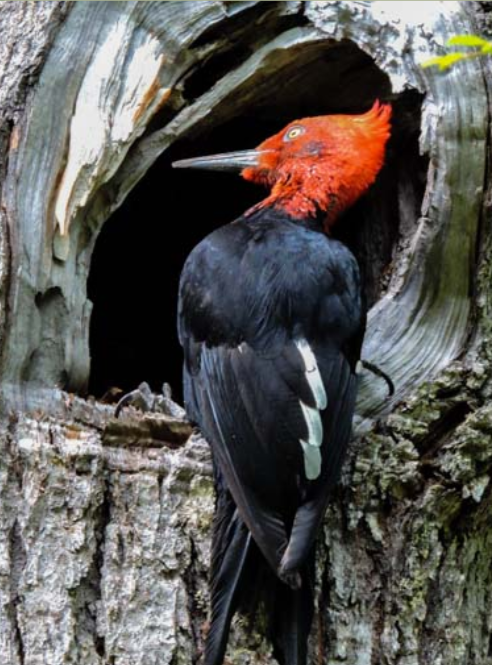
\includegraphics[width=0.4\linewidth]{ImagenesIntroduccion/pajaro}
	\label{fig:pajaro}
	\caption{Imagen del ave.}
\end{figure}

Durante los meses de primavera, estas aves entran en lo que se llama periodo de anidación, donde la hembra pone hasta 4 huevos. A lo largo de este intervalo, el macho y la hembra se turnan para incubar. Los primeros se hacen cargo durante la noche (aproximadamente 6 a 8 horas), mientras que las segundas se ocupan durante el día. Es fundamental saber que esta especie actúa de forma muy agresiva y territorial durante este tiempo, ya que buscan proteger a su descendencia.

Otro aspecto vital es conocer la morfología del nido, lugar donde van los sensores del proyecto. Debido a los hábitos de limpieza del ave, el único lugar factible para la posición de la electrónica resulta ser la bóveda del nido.
\begin{figure}[H]
	\centering
	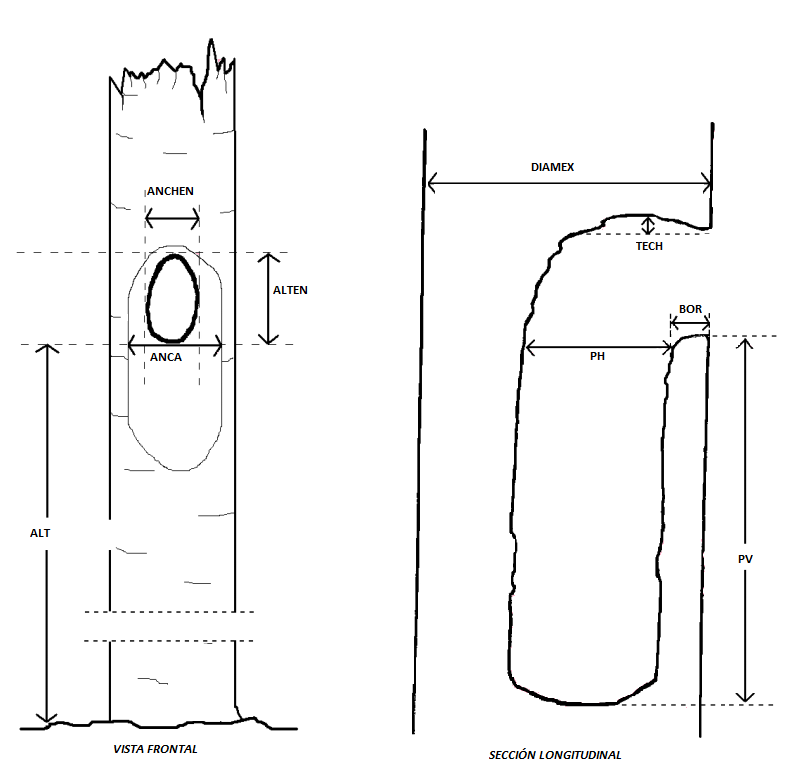
\includegraphics[width=0.5\linewidth]{ImagenesIntroduccion/morfologia_nido}
	\label{fig:morfología_nido}
	\caption{Morfología nido.}
\end{figure}

\begin{table}[H]
\centering
\begin{tabular}{|c|c|c|c|}
\hline
\textbf{Variable}    & \textbf{Media} & \textbf{Rango}     & \textbf{Muestras} \\ \hline
\textbf{DIAMEX [cm]} & 45.56          & 33.74 $\sim$ 71.94 & 26                \\ \hline
\textbf{ANCA [cm]}   & 23.41          & 18.3 $\sim$ 33     & 26                \\ \hline
\textbf{ALT [m]}     & 8.68           & 3.3 $\sim$ 17      & 27                \\ \hline
\textbf{ANCHEN [cm]} & 8.79           & 7.9 $\sim$ 9.7     & 27                \\ \hline
\textbf{ALTEN [cm]}  & 15.40          & 11.4 $\sim$ 20     & 27                \\ \hline
\textbf{PV [cm]}     & 32.52          & 21 $\sim$ 44       & 27                \\ \hline
\textbf{PH [cm]}     & 26.22          & 20 $\sim$ 33       & 27                \\ \hline
\textbf{BOR [cm]}    & 6.41           & 4 $\sim$ 12        & 27                \\ \hline
\textbf{TECH [cm]}   & 4.55           & 0 $\sim$ 10        & 27                \\ \hline
\end{tabular}
\caption{Medidas del nido.}
\end{table}

Además de esta información, se sabe que el grupo de investigadores se presentan cada dos semanas en la base del árbol, frente al nido, para obtener la información recolectada por el dispositivo.

Finalmente cabe mencionar que este proyecto es complementario de otro ajeno, el cual involucra una mochila que se encuentra sobre el pájaro. Este equipamiento busca obtener datos propios del ave, de su posición y trayectoria. Es por eso que cobra importancia el comportamiento de la especie durante el anidamiento.

La importancia de este complemento es que la información que recolecte debe ser transmitida y almacenada en el nido, unificando así ambos proyectos al momento de brindarle acceso al usuario. 

Otro aspecto que se debe contemplar con respecto a la mochila es que debe proponerse la viabilidad energética de esta. En otras palabras, se deben plantear propuestas que garanticen el funcionamiento del dispositivo a lo largo del proceso de investigación.

%\end{document}